\documentclass[12pt, titlepage]{article}

\usepackage{xcolor} % for different colour comments
\usepackage{tabto}
\usepackage{mdframed}
\mdfsetup{nobreak=true}
\usepackage{xkeyval}
\usepackage{tabularx}
\usepackage{booktabs}
\usepackage{hyperref}
\hypersetup{
    colorlinks,
    citecolor=black,
    filecolor=black,
    linkcolor=red,
    urlcolor=blue
}
\usepackage[skip=2pt, labelfont=bf]{caption}
\usepackage{titlesec}
\usepackage{placeins}
\usepackage{graphicx}
\graphicspath{ {image/} }




%% the following adds another section level by redefining the paragraph
%% source:  http://tex.stackexchange.com/questions/60209/how-to-add-an-extra-level-of-sections-with-headings-below-subsubsection
\setcounter{secnumdepth}{4}

\titleformat{\paragraph}
{\normalfont\normalsize\bfseries}{\theparagraph}{1em}{}
\titlespacing*{\paragraph}
{0pt}{3.25ex plus 1ex minus .2ex}{1.5ex plus .2ex}


%% Comments
\newif\ifcomments\commentstrue

\ifcomments
\newcommand{\authornote}[3]{\textcolor{#1}{[#3 ---#2]}}
\newcommand{\todo}[1]{\textcolor{red}{[TODO: #1]}}
\else
\newcommand{\authornote}[3]{}
\newcommand{\todo}[1]{}
\fi

\newcommand{\wss}[1]{\authornote{magenta}{SS}{#1}}
\newcommand{\ds}[1]{\authornote{blue}{DS}{#1}}



%% The following are used for pretty printing of events and requirements
\makeatletter

\define@cmdkey      [TP] {test}     {name}       {}
\define@cmdkey      [TP] {test}     {desc}       {}
\define@cmdkey      [TP] {test}     {type}       {}
\define@cmdkey      [TP] {test}     {init}       {}
\define@cmdkey      [TP] {test}     {input}      {}
\define@cmdkey      [TP] {test}     {output}     {}
\define@cmdkey      [TP] {test}     {pass}       {}
\define@cmdkey      [TP] {test}     {user}       {}


\newcommand{\getCurrentSectionNumber}{%
  \ifnum\c@section=0 %
  \thechapter
  \else
  \ifnum\c@subsection=0 %
  \thesection
  \else
  \ifnum\c@subsubsection=0 %
  \thesubsection
  \else
  \thesubsubsection
  \fi
  \fi
  \fi
}

\newcounter{TestNum}

%\@addtoreset{TestNum}{section}
%\@addtoreset{TestNum}{subsection}
%\@addtoreset{TestNum}{subsubsection}



\newcommand{\testauto}[1]{
\setkeys[TP]{test}{#1}
\refstepcounter{TestNum}
\begin{mdframed}[linewidth=1pt]
\begin{tabularx}{\textwidth}{@{}p{3cm}X@{}}
{\bf Test \#\theTestNum:} & {\bf \cmdTP@test@name}\\[\baselineskip]
{\bf Description:} & \cmdTP@test@desc\\[0.5\baselineskip]
{\bf Type:} & \cmdTP@test@type\\[0.5\baselineskip]
{\bf Initial State:} & \cmdTP@test@init\\[0.5\baselineskip]
{\bf Input:} & \cmdTP@test@input\\[0.5\baselineskip]
{\bf Output:} & \cmdTP@test@output\\[0.5\baselineskip]
{\bf Pass:} & \cmdTP@test@pass
\end{tabularx}
\end{mdframed}
}

\newcommand{\testautob}[1]{
\setkeys[TP]{test}{#1}
\refstepcounter{TestNum}
\begin{mdframed}[linewidth=1pt]
\begin{tabularx}{\textwidth}{@{}p{3cm}X@{}}
{\bf Test \#\theTestNum:} & {\bf \cmdTP@test@name}\\[\baselineskip]
{\bf Description:} & \cmdTP@test@desc\\[0.5\baselineskip]
{\bf Type:} & \cmdTP@test@type\\[0.5\baselineskip]
{\bf Pass:} & \cmdTP@test@pass
\end{tabularx}
\end{mdframed}
}

\newcommand{\testmanual}[1]{
\setkeys[TP]{test}{#1}
\refstepcounter{TestNum}
\begin{mdframed}[linewidth=1pt]
\begin{tabularx}{\textwidth}{@{}p{3cm}X@{}}
{\bf Test \#\theTestNum:} & {\bf \cmdTP@test@name}\\[\baselineskip]
{\bf Description:} & \cmdTP@test@desc\\[0.5\baselineskip]
{\bf Type:} & \cmdTP@test@type\\[0.5\baselineskip]
{\bf Tester(s):} & \cmdTP@test@user\\[0.5\baselineskip]
{\bf Pass:} & \cmdTP@test@pass
\end{tabularx}
\end{mdframed}
}


\makeatother

\newcommand{\ZtoT}{
\begin{tabularx}{3.85cm}{@{}p{0.35cm}p{0.35cm}p{0.35cm}p{0.35cm}p{0.35cm}p{0.35cm}p{0.35cm}p{0.35cm}p{0.35cm}p{0.35cm}p{0.35cm}@{}}
0 & 1 & 2 & 3 & 4 & 5 & 6 & 7 & 8 & 9 & 10
\end{tabularx}
}

\begin{document}
\title{\bf Platform Perils\\[\baselineskip]\Large Test Plan}
\author{Steven Palmer\\$\langle$palmes4$\rangle$\\Chao Ye\\$\langle$yec6$\rangle$}
\date{\today}
	
\maketitle

\pagenumbering{roman}
\tableofcontents
\listoftables
\listoffigures


\begin{table}[bp]
\caption*{\bf Revision History}
\begin{tabularx}{\textwidth}{p{3.5cm}p{2cm}X}
\toprule {\bf Date} & {\bf Version} & {\bf Notes}\\
\midrule
October 25, 2015 & 1.0 & Created document\\
October 31, 2015 & 1.1 & Major additions to all sections\\
November 1, 2015 & 1.2 & Final version for rev 0\\
April 25, 2015 & 1.3 & Final version for rev 1\\
\bottomrule
\end{tabularx}
\end{table}

\newpage

\pagenumbering{arabic}

\section{Overview}
The purpose of this document is to provide a detailed plan for the testing of our game.  The following brief outline gives an overview of what is covered in this document:

\begin{itemize}
  \item A proof of concept test is described in \hyperref[sec:poc]{\S\ref*{sec:poc}}.
  \item The set of tests that will be used in testing the system is described in \hyperref[sec:testing]{\S\ref*{sec:testing}}.
  \item The set of tests that will be used to ensure that the software requirements specifications are met is described in \hyperref[sec:reqtesting]{\S\ref*{sec:reqtesting}}.
  \item A timeline of the test plan is given in \hyperref[sec:timeline]{\S\ref*{sec:timeline}}.
\end{itemize}

\subsection{Test Case Format}
The description of the tests that will be carried out are formatted in the following way throughout the document:

\begin{mdframed}[linewidth=1pt]
\begin{tabularx}{\textwidth}{@{}p{3cm}X@{}}
{\bf Test \#:} & {\bf Test name}\\[\baselineskip]
{\bf Description:} & A description of what is being tested\\[0.5\baselineskip]
{\bf Type:} & The type of test\\[0.5\baselineskip]
{\bf Tester(s):} & The people who will run the test ({\bf manual only})\\[0.5\baselineskip]
{\bf Initial State:} & The initial state of the system being tested ({\bf unit test only})\\[0.5\baselineskip]
{\bf Input:} &  The input that will change the state of the system ({\bf unit test only})\\[0.5\baselineskip]
{\bf Output:} & The relevant output that is checked ({\bf unit test only})\\[0.5\baselineskip]
{\bf Pass:} & The pass criteria for the relevant output in the case of unit tests, or a description of the pass criteria for other tests
\end{tabularx}
\end{mdframed}

\subsection{Automated Testing}
Automated testing will be used for testing of the game mechanics system and will be carried out via unit test suites.  Stubs and drivers will not be used due to the heavy use of side-effects in game code.  To ensure that unit testing can be run while the game mechanics are in development the test cases have been grouped into sections that can be fully implemented once certain subsets of the game mechanics systems are completed.

\subsubsection{Testing Tools}
The software tools that will be used to carry out the automated testing are listed in \hyperref[tab:tools]{Table~\ref*{tab:tools}}.

\begin{table}[ht]
\caption{List of testing tools} \label{tab:tools}
\begin{tabularx}{\textwidth}{p{2.3cm}p{4.5cm}X}
\toprule {\bf Tool} & {\bf Description} & {\bf Use}\\
\midrule
gUnit & Unit testing framework & Unit testing\\
\bottomrule
\end{tabularx}
\end{table}

\subsection{Manual Testing}
Manual tests will be used for testing all aspects of the game that are not covered by the automated unit testing suite (the time that would be required to develop automated tests for these test cases would be prohibitive).  The game development team will carry out these tests as the game is developed.


\subsection{List of Constants}
Constants used in this document are listed in \hyperref[tab:constants]{Table~\ref*{tab:constants}}.
\begin{table}[ht]
\caption{List of constants} \label{tab:constants}
\begin{tabularx}{\textwidth}{p{3cm}p{2cm}X}
\toprule {\bf Constant} & {\bf Value} & {\bf Description}\\
\midrule
$\sigma$ & 60 & Frame rate target\\
$\delta$ & 3 & Number of people in user testing group\\
$\Theta$ & 6 & User testing entertainment target\\
$\Psi$ & 2 & User testing challenge range\\
$\Omega$ & 8 & User testing controls target\\
$\Phi$ & 250 & Dynamic object limit\\
\bottomrule
\end{tabularx}
\end{table}

\newpage
\section{Proof of Concept Testing}
\label{sec:poc}
Before any serious development of the game begins, a proof of concept test will be carried out to show that the undertaking is feasible.  The remainder of this section describes the proof of concept test in detail.

\subsection{Significant Risks}
The successful completion of the project depends on overcoming the following significant risks:
\begin{enumerate}
  \item In order to use the Chipmunk2D library it must first be successfully compiled.  Since we intend for the game to be compatible with Windows 7, Mac OS X, and Ubuntu, there is a significant risk for the project to fail if compilation is not achieved on all three operating systems.
  \item Chipmunk2D is a large library and its use is not straight forward.  Successful implementation of the library features is crucial to the success of the project and the failure of this poses another significant risk.
\end{enumerate}


\subsection{Demonstration Plan}

For a proof of concept test we will produce a working prototype that can be run on Windows 7, Mac OS X, and Ubuntu.  The prototype will consist of a game demo that implements gravity and collision detection provided by the Chipmunk2D library.  Rudimentary graphics will be used for the prototype since the scope is limited only to demonstrating that the identified risks can be overcome.

The prototype will consist of a small room in which a hero character and enemies exist.  The room will be bounded by a floor below and walls on the left and right, all of which the hero and enemies cannot pass through.  The room will contain platforms which the hero and enemies cannot pass through from above, but may pass through from below when jumping.  A rough idea of the room is given in \hyperref[fig:room]{Figure~\ref*{fig:room}}.

\begin{figure}[ht]
\centering
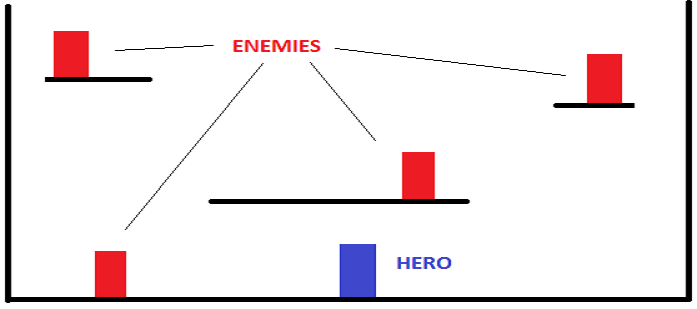
\includegraphics[width=0.75\textwidth]{demo}
\caption{Proof of concept sketch} \label{fig:room}
\end{figure}

The hero character will be represented by a blue rectangle and will be controlled by the user in the following ways:

\begin{itemize}
  \item The hero moves left and right using the 'a' and 'd' keys respectively
  \item The hero jumps by pressing the 'space' key
  \item The hero shoots a projectile in the direction of the mouse cursor by left-clicking
\end{itemize}

Enemies will be represented by red rectangles and will not have any programmed AI (they will not move or attack).  The hero will be able to attack enemies with a projectile, which will knock them back when they are hit.  The hero and all enemies will be subject to gravity and will free-fall when there is no platform or boundary under them.

The proof of concept is given in test case format to adhere with the presentation of the other tests in this document.
\testmanual{
    name = Proof of Concept,
    desc = Tests whether significant risks to the completion of the project can be overcome,
    type = {Proof of Concept (manual)},
    user = Game developers,
    pass = {Successful development of a small demonstration which makes use of the Chipmunk2D physics engine and runs on Windows 7, Mac OS X, and Ubuntu}
}

\section{System Testing}
\label{sec:testing}
The testing of the system is broken down into game mechanics testing and game design testing phases.  The game mechanics will be developed and tested first.  Once the game mechanics systems are in place, the game design development and testing phase will begin.




\subsection{Game Mechanics Testing}
\label{sec:mechanicstesting}
\subsubsection{Automated Testing}
A limited set of unit tests will be used to test the game mechanics and physics.  This test suite will be used to ensure that changes to the game do not break the basic functioning of the game.  The test cases that will be used are outlined in the remainder of this section.

\testauto{
    name = {Move left},
    desc = Tests if the hero moves left when the corresponding input is received when the hero is initially stationary,
    type = {Unit Test (dynamic, automated)},
    init = Custom in-game state with a hero object having x-velocity of zero,
    input = Keyboard function called with simulated left key down stroke,
    output = Hero object x-velocity,
    pass = Hero object x-velocity is less than zero
}

\testauto{
    name = {Move right},
    desc = Tests if the hero moves right when the corresponding input is received when the hero is initially stationary,
    type = {Unit Test (dynamic, automated)},
    init = Custom in-game state with hero object having x-velocity of zero,
    input = Keyboard function called with simulated right key down stroke,
    output = Hero object x-velocity,
    pass = Hero object x-velocity is greater than zero
}

\testauto{
    name = Stop moving left,
    desc = Tests if hero stops moving left when corresponding input is stopped,
    type = {Unit Test (dynamic, automated)},
    init = Custom in-game state with hero object having x-velocity less than zero,
    input = Keyboard function called with simulated left key up stroke,
    output = Hero object x-velocity,
    pass = Hero object x-velocity is zero
}

\testauto{
    name = Stop moving right,
    desc = Tests if hero stops moving right when corresponding input is stopped,
    type = {Unit Test (dynamic, automated)},
    init = Custom in-game state with hero object having x-velocity greater than zero,
    input = Keyboard function called with simulated right key up stroke,
    output = Hero object x-velocity,
    pass = Hero object x-velocity is zero
}

\testauto{
    name = Jump from static object,
    desc = Tests if hero jumps off a static object when corresponding input is received,
    type = {Unit Test (dynamic, automated)},
    init = Custom in-game state with hero object having y-velocity of zero and a bottom edge in contact with a static object,
    input = Keyboard function called with simulated space bar key down stroke,
    output = Hero object y-velocity,
    pass = Hero object y-velocity is greater than zero
}

\testauto{
    name = Wall obstructs hero moving left,
    desc = Tests whether the hero is stopped by a wall object while moving left,
    type = {Unit Test (dynamic, automated)},
    init = Custom in-game state with hero object having x-velocity less than zero situated directly to the right of a wall object,
    input = The chipmunk cpSpaceStep function is called,
    output = Hero object x-velocity,
    pass = Hero object x-velocity is 0
}

\testauto{
    name = Wall obstructs hero moving right,
    desc = Tests whether the hero is stopped by a wall object while moving right,
    type = {Unit Test (dynamic, automated)},
    init = Custom in-game state with hero object having x-velocity greater than zero situated directly to the left of a wall object,
    input = The chipmunk cpSpaceStep function is called,
    output = Hero object x-velocity,
    pass = Hero object x-velocity is 0
}

\testauto{
    name = Floor supports stationary hero,
    desc = Tests whether the hero is supported by a floor object,
    type = {Unit Test (dynamic, automated)},
    init = Custom in-game state with stationary hero object situated directly on top of a floor object,
    input = The chipmunk cpSpaceStep function is called,
    output = Hero object y-velocity,
    pass = Hero object y-velocity is 0
}

\testauto{
    name = {Floor stops hero in free fall},
    desc = Tests whether the hero in free fall is stopped by a floor object,
    type = {Unit Test (dynamic, automated)},
    init = Custom in-game state with hero object with y-velocity less than zero situated directly on top of a floor object,
    input = The chipmunk cpSpaceStep function is called,
    output = Hero object y-velocity,
    pass = Hero object y-velocity is 0
}


\subsubsection{Manual Testing}
The following manual tests will be carried out to provide testing for game mechanics related requirements that are not covered by unit tests.

\testmanual{
    name = No mid-air jumps,
    desc = Tests that the hero cannot jump when not in contact with a surface,
    type = {Functional (dynamic, manual)},
    user = {Development team},
    pass = Hero cannot jump when not in contact with a surface
}

\testmanual{
    name = Zoom in test,
    desc = Tests that the stage zooming works properly (in),
    type = {Functional (dynamic, manual)},
    user = {Development team},
    pass = Stage view can be zoomed in
}

\testmanual{
    name = Zoom out test,
    desc = Tests that the stage zooming works properly (out),
    type = {Functional (dynamic, manual)},
    user = {Development team},
    pass = Stage view can be zoomed out
}

\testmanual{
    name = Hero death,
    desc = Tests that the hero is killed when coming into contact with a fatal hazard,
    type = {Functional (dynamic, manual)},
    user = {Development team},
    pass = Hero is killed when contacting fatal hazards
}

\testmanual{
    name = Stage win,
    desc = Tests that the stage is won when hero comes in contact with the checkered goal,
    type = {Functional (dynamic, manual)},
    user = {Development team},
    pass = Stage is won and user is returned to the main menu
}

\testmanual{
    name = General physics behaviour,
    desc = Tests that the physics behaves as expected from a qualitative perspective,
    type = {Functional (dynamic, manual)},
    user = {Development team},
    pass = Physics appears to function correctly
}

\testmanual{
    name = General collision behaviour,
    desc = Tests that collisions behave as expected from a qualitative perspective,
    type = {Functional (dynamic, manual)},
    user = {Development team},
    pass = Collisions appear to behave correctly
}



\subsection{Game Design Testing}
Once the game mechanics systems have been implemented and shown to be working correctly through the testing described in \hyperref[sec:mechanicstesting]{\S\ref*{sec:mechanicstesting}}, the game itself will be built on top.  The design of the game can be broken down into the design of the game world, graphics, and sound.  Automated testing for this phase would be time-consuming and difficult to implement.  Therefore, all of the game design testing will consist of manual tests.
\subsubsection{Game World Testing}
The following tests will be carried out to ensure that the game world is designed correctly.

\testmanual{
    name = All areas reachable,
    desc = Tests that all areas of the game world that are intended to be reachable by the hero are in fact reachable by the hero,
    type = {Functional (dynamic, manual)},
    user = {Development team},
    pass = No areas are unreachable based on a thorough playthrough testing of the game
}

\testmanual{
    name = No ``points of no return'',
    desc = Tests that there are no areas of the game world that will cause the hero to become stuck (e.g. inescapable pits),
    type = {Functional (dynamic, manual)},
    user = {Development team},
    pass = There are no inescapable areas detected on a thorough playthrough testing of the game
}

\subsubsection{Graphics Testing}
The following tests will be carried out to ensure that the game graphics are properly implemented.

\testmanual{
    name = Textures,
    desc = Tests if textures are properly implemented,
    type = {Functional (dynamic, manual)},
    user = Development team,
    pass = {In-game textures appear correct by inspection}
}

\testmanual{
    name = Lighting,
    desc = Tests if lighting effects are properly implemented,
    type = {Functional (dynamic, manual)},
    user = Development team,
    pass = {Lighting effects appear correct by inspection}
}


\subsubsection{Audio Testing}
The following tests will be carried out to ensure that the game audio is properly implemented.

\testmanual{
    name = Background music,
    desc = Tests if background music is properly implemented,
    type = {Functional (dynamic, manual)},
    user = Development team,
    pass = {Background music plays while in game}
}

\testmanual{
    name = Sound effects,
    desc = Tests if sound effects are properly implemented,
    type = {Functional (dynamic, manual)},
    user = Development team,
    pass = {Appropriate sounds play when events take place (e.g. hero death, complete stage)}
}

\subsubsection{Miscellaneous Testing}
The following tests will be carried out to ensure all requirements not tested under the previous categories are met.

\testmanual{
    name = Menu system,
    desc = {The menu system works as intended},
    type = {Functional (dynamic, manual)},
    user = {Development team},
    pass = All menu options work correctly,
}

\testmanual{
    name = General look and feel,
    desc = {The game has the intended look and feel},
    type = {Functional (dynamic, manual)},
    user = {Development team},
    pass = The game is a 2.5-D platformer with an Indiana Jones adventure theme,
}

\testmanual{
    name = Operating system support,
    desc = {The game runs on Windows 7, Mac OS X, and Ubuntu},
    type = {Functional (dynamic, manual)},
    user = {Development team},
    pass = Game can be compiled and system tests all pass on each platform,
}

\testmanual{
    name = Spelling and grammar check,
    desc = The game uses proper English and is free of any spelling or grammatical errors,
    type = {Functional (dynamic, manual)},
    user = {Development team},
    pass = No spelling or grammatical errors are detected (or all detected errors are corrected)
}

\testmanual{
    name = Hardware requirements,
    desc = Tests for the minimum hardware requirements required to maintain an average frame rate of at least $\hyperref[tab:constants]{\sigma}$ frames per second,
    type = {Functional (dynamic, manual)},
    user = {Development team},
    pass = Game maintains frame rate of at least $\hyperref[tab:constants]{\sigma}$ frames per second in a stage that contains $\hyperref[tab:constants]{\Phi}$ dynamic objects when tested on a low-performance system
}


\section{Future Testing}
\subsection{User Experience Testing}
\label{sec:userexp}
User experience testing will be completed by a testing group consisting of $\hyperref[tab:constants]{\delta}$ individuals who were not involved in the development of the game.  The testing group will be given a copy of the game and asked to complete a survey (see \hyperref[sec:survey]{Appendix A}) after having played the game to provide feedback.  Due to time constraints, these tests will be carried out subsequent to the revision 1 project submission.

\testmanual{
    name = {Entertainment},
    desc = Tests that the game is entertaining,
    type = {Functional (dynamic, manual)},
    user = {Testing group},
    pass = {Average survey score of at least $\hyperref[tab:constants]{\Theta}$}
}

\testmanual{
    name = {Challenge},
    desc = Tests that the game is adequately challenging (not too easy or too hard),
    type = {Functional (dynamic, manual)},
    user = {Testing group},
    pass = {Average survey score within $\hyperref[tab:constants]{\Psi}$ of 5}
}

\testmanual{
    name = {Controls},
    desc = Tests that the game controls are intuitive,
    type = {Functional (dynamic, manual)},
    user = {Testing group},
    pass = {Average survey score of at least $\hyperref[tab:constants]{\Omega}$}
}

\section{Trace to Requirements}
\label{sec:reqtesting}



\subsection{Functional Requirements}
A trace between tests and functional requirements is provided in \hyperref[tab:reqtrace]{Table~\ref*{tab:reqtrace}}.

\begin{table}[h]
\caption{\bf Requirements Traceability} \label{tab:reqtrace}
\centering
\begin{tabularx}{0.55\textwidth}{p{4cm}X}
\toprule {\bf Requirement} & {\bf Test(s)}\\
\midrule
1	&	24	\\
2	&	24	\\
3	&	24	\\
4	&	24	\\
5	&	2, 4	\\
6	&	3, 5	\\
7	&	6	\\
8	&	11	\\
9	&	16\\
10	&	19	\\
11	&	18	\\
12	&	12	\\
13	&	13	\\
14	&	9, 10	\\
15	&	7, 8	\\
16	&	14, 17	\\
17	&	14	\\
18	&	15	\\
19	&	24	\\
20	&	25	\\
21	&	25	\\
22	&	20, 21, 25	\\
23	&	22, 23	\\
24	&	29	\\
25	&	31	\\
26	&	30	\\
27	&	28	\\
28  &    26   \\
29  &    27   \\
\bottomrule
\end{tabularx}
\end{table}


\FloatBarrier 
\section{Timeline}
\label{sec:timeline}
This document is structured to roughly match the anticipated chronology of testing.  The testing timeline is given in \hyperref[tab:timeline]{Table~\ref*{tab:timeline}}.


\begin{table}[ht]
\caption{Testing timeline} \label{tab:timeline}
\begin{tabularx}{\textwidth}{p{2.5cm}p{3cm}X}
\toprule {\bf Completion Date} & {\bf Responsible Party} & {\bf Task}\\
\midrule
11/15/2015 & Development team & Completion of the proof of concept demo\\[0.3\baselineskip]
04/15/2016 & Chao Ye & Implementation of input unit test cases\\[0.3\baselineskip]
04/15/2016 & Chao Ye & Implementation of collision unit test cases\\[0.3\baselineskip]
04/18/2016 & Steven Palmer & Completion of game design testing\\[0.3\baselineskip]
Future & Testing group & Completion of user experience survey\\
\bottomrule
\end{tabularx}
\end{table}

\FloatBarrier
\newpage
\section{Appendix A:  Testing Survey}
\label{sec:survey}

The following survey will be filled out by members of the alpha and beta testing groups.

\begin{mdframed}[linewidth=1pt]
\begin{center}
{\bf \large User Experience Survey}\\[\baselineskip]
\end{center}

\noindent The following survey should be filled out after playing the game for at least 30 minutes.\\

\noindent {\bf Time played:}\\

\noindent Please provide a ranking between 0 and 10 in each of the following categories.  Please include notes on what you did and did not like, and what could be done to improve the game.\\[\baselineskip]

\noindent \begin{tabularx}{\textwidth}{@{}p{3.5cm}X@{}}
{\bf Entertainment:} & \ZtoT \\
& {[~0 = most boring, 10 = most fun~]}\\[\baselineskip]
{\bf Difficulty:} & \ZtoT\\
& {[~0 = easiest, 10 = most difficult~]}\\[\baselineskip]
{\bf Controls:} & \ZtoT\\
& {[~0 = non-intuitive, 10 = intuitive~]}\\[\baselineskip]
{\bf Notes:} & \\[5\baselineskip]
\end{tabularx}
\end{mdframed}



\end{document}
